	El núcleo del Kit de Desarrollo FX2LP EZ-USB es un CY7C68013A. Dicho circuito integrado, cuya arquitectura se presenta en la Figura \ref{arqEzUSB}, pertenece a la serie FX2LP de la familia de integrados EZ-USB comercializado por Cypress Semiconductors.\\
	
	Esta serie se caracteriza por brindar una conexión USB 2.0 de alta velocidad y bajo consumo energético, especialmente diseñados para productos con autonomía limitada. Se integra un controlador USB completo, incluyendo un transceptor USB, un MIS (Motor de Interfaz Serial), buffers de datos implementados con memorias tipo FIFO (\(First In First Out\); Primero Entrado, Primero Salido), un microcontrolador 8051 mejorado y una interfaz programable hacia los periféricos. Además posee un PLL con divisor configurable a través de los cuales proveen las señales de reloj adecuadas para el correcto funcionamiento del sistema.\\
	
	\begin{figure}[b]
		\centering
		%TODO meter la imagen
		\begin{tikzpicture}[scale=\textwidth/\paperwidth]
			\begin{scope}[
				>=latex,
				node distance=1,
				align=center,
				transform shape
				]
				\node			(aux1)	[]				{};
				\node[core,
				minimum height=95]
				(mis)	[left=of aux1,anchor=north east]	{MIS};
				\node[core]		(ram)	[right=of aux1,anchor=north west, text width=30]	{16 kB RAM};
				\node[perif,
				text width=60]
				(xcvr)	[left=of mis]	{Transceptor USB};
				\node[interior,
				minimum size=60,
				text width=50]
				(uc)	[above=of aux1]	{8051 Mejorado};			
				\node[perif,
				node distance=2.9]
				(pll)	[left=of uc]	{PLL};
				
				\node			(aux2)	[right=of ram.south]{};				
				\node[core,
					text width=120]
								(bus)	[right=of aux2,rotate=90,anchor=north west]	{Bus de datos y direcciones};
				
				\node[perif]	(i2c)	[right=of bus.south east,anchor=north west]	{I2C};
				\node[perif,
					text width=30]
								(gpif)	[right=of bus.south west,anchor=south west] {GPIF};
				\node[perif,
				text width=40]
				(fifo)	[below=of gpif]	{4 kB FIFO};
				\node 			(aux3)	[right=of fifo]	{};
				\node 			(aux5) 	[left=of ram] {};
				
				\draw[<->]	(mis) -- (xcvr);
				\draw[<->]	(ram) -- (ram -| mis.east);
				\draw[<->]	(fifo) -- (fifo -| mis.east);
				\draw[<->]	(ram) to (ram -| bus.north);
				\draw[<->]	(uc) to (uc -| bus.north);
				\draw[<-]	(xcvr) to (xcvr |- pll.south);
				\draw[->]	(pll) to (uc);
				\draw[<->]	(i2c) to (i2c -| bus.south);
				\draw[<->]	(gpif) to (gpif -| bus.south);
				\draw[]		(fifo) -| (aux5.center);
			\end{scope}
			
			\begin{scope}[on background layer]
				\node[contenedor] (fx2) [fit=(pll)(xcvr)(uc)(bus)(mis)(ram)(fifo)(gpif)(i2c)(aux3)]{};
			\end{scope}
			
			\begin{scope}[
				transform shape,
				>=latex
				]
				\node[text width=40,align=center]	(xtal)	[left=of pll]{Xtal \SI{24}{\mega\hertz}};
				\node	(host)	[left=3of xcvr]	{PC};
				\draw[<->,ultra thick] (host) -- node [above,text width=70,midway,align=center]{Comunicación USB} (xcvr);
				\draw[->] (xtal) to (pll);
				\draw[<->,ultra thick] (bus.240) -- node [above,align=center,text width=80] {Datos, direcciones y entradas adicionales}(bus.240 -| fx2.east);
				\draw[<->,thick] (gpif) to (gpif -| fx2.east);
				\draw[<->,thick] (fifo) to (fifo -| fx2.east);
				\draw[<->,thick] (i2c) to (i2c -| fx2.east);
			\end{scope}
		\end{tikzpicture}
%		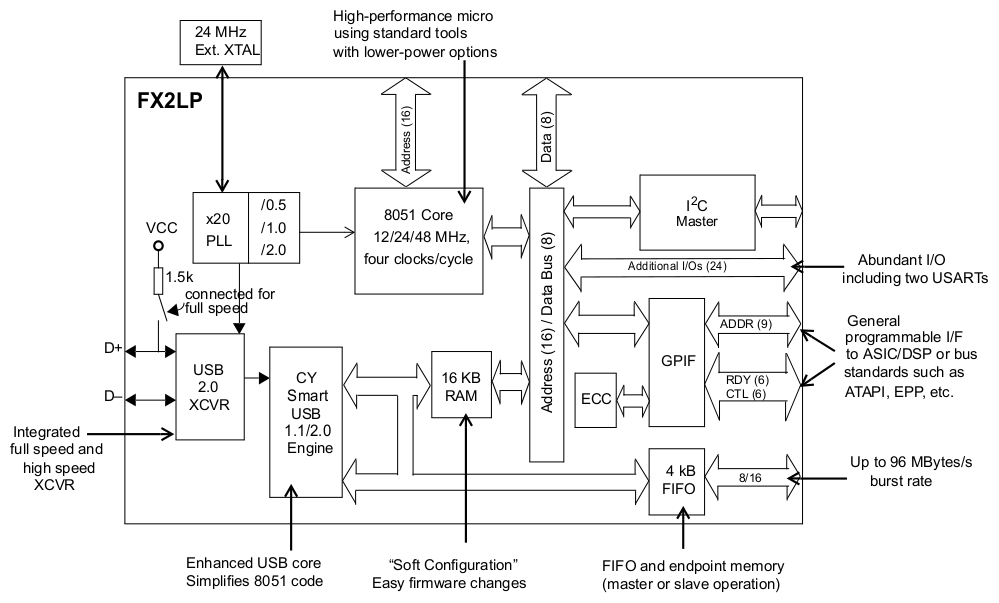
\includegraphics[width=.7\textwidth]{arqfx2lp.png}
%		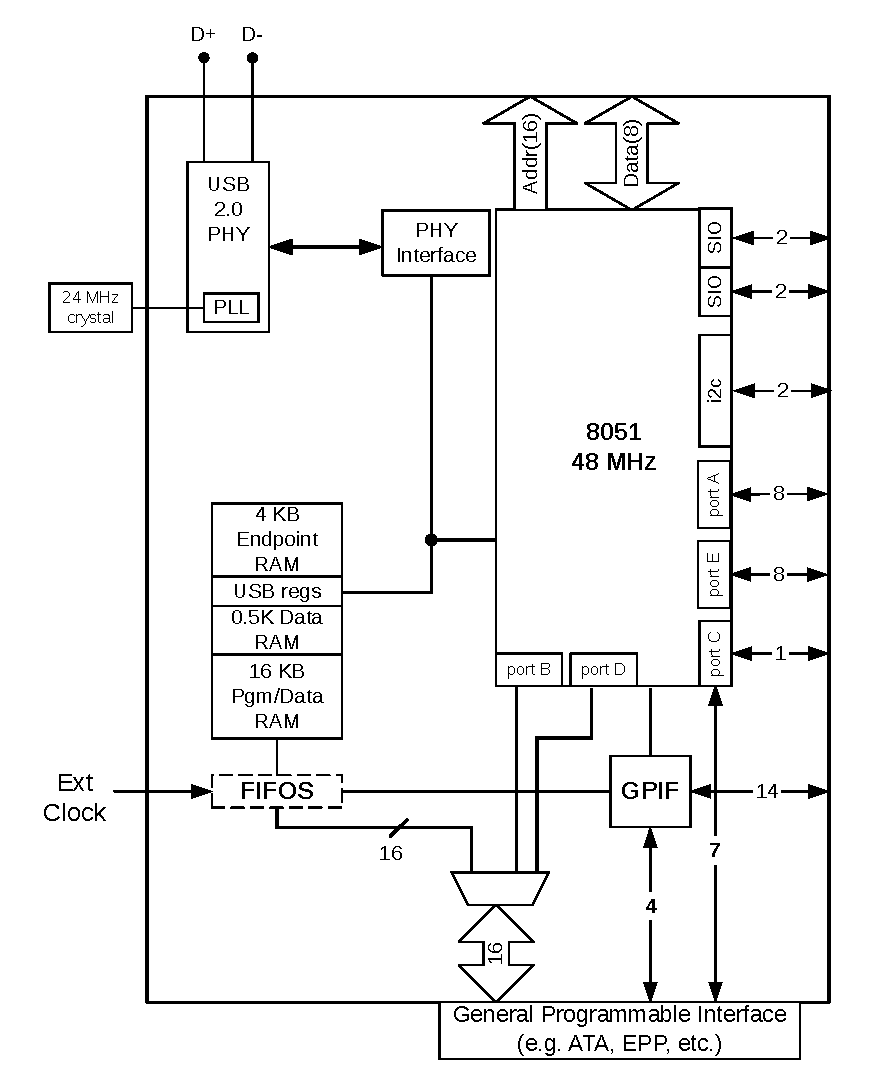
\includegraphics[width=.55\textwidth]{arq.eps}
		%TODO Meter la referencia
		\caption{Arquitectura FX2LP} 
		\label{arqEzUSB}
	\end{figure}

	De esta forma, se permite al usuario trasmitir datos desde y hacia el anfitrión a través del  mismo puerto USB, o bien via RS-232. Para comunicarse con sistemas periféricos se puede aprovechar el puerto $I^2C$, la interfaz de propósito general, que actúa como maestro y a la cual se le puede acoplar un periférico esclavo, y/o las memorias FIFO en modo esclavo que puede ser conectada a un sistema maestro. Esto brinda muchas alternativas, desde la conexión a puertos estandar, como ser ATA, PCMCIA, EPP, etc. o también la conexión de dispositivos tales como DSP's y FPGA's.\\
	
	Este trabajo utiliza particularmente las memorias FIFO en modo esclavo, que responden a las diferentes señales que les proporciona un maestro externo implementado con un FPGA; por lo que a continuación se explicitan algunos detalles referidos a ellos, con lo que se busca aclarar el funcionamiento y que el lector comprenda los fundamentos de las configuraciones que se plasmarán en el código del firmware.\\
	
	\subsection{Motor de Interfaz Serial}
	
		La comunicación USB se realiza a través del transceptor, unido al MIS. Como se observa en la Figura \ref{usbxcvr}, el usuario, a fin de intercambiar datos, solo debe colocar o extraer los datos de registros destinados a tal fin y modificar las banderas de handshaking, que en la figura se observan como ACK (abreviación del ingles {\it acknowledge}, que significa reconocer, aceptar o agradecer), que indican si el sistema está disponible, si los datos fueron colocados o leídos, dependiendo el caso tratado. De forma automática, el MIS y el transceptor USB se encargan de empaquetar, enviar, recibir y desempaquetar toda la información, así como leer los tokens que emite el host, calcular y corroborar los códigos cíclicos de detección de errores y todo lo relacionado al protocolo propiamente dicho.\\
	
		\begin{figure}[hb]
			\centering
			\includegraphics[width=.8\textwidth]{usbxcvr}
			\caption{Implementación del enlace USB realizado por el EZ-USB}
			\label{usbxcvr}
		\end{figure}
	
	\subsection{Modos de entrada y salida automáticos}
	
		Los datos que se reciben o envían a través del MIS. Tal como se observa en al Figura \ref{modesfifo}, pueden ser enviados en forma automatica desde y hacia las memorias FIFO, o bien, pueden ser dirigidos a través del microcontrolador. Esto último permite leer, modificar, suprimir, agregar y/o generar nuevos datos antes de ser remitido el paquete a su respectivo extremo.\\
	
		Los fabricantes llaman a estos caminos "MODO MANUAL", en caso de enviar los datos a través del 8051, y "MODO AUTOMÁTICO", cuando la comunicación es directa entre el MIS y las FIFO. Además, son configurables independientemente para cada extremo, sea este de salida o entrada.\\
	
		Se debe notar en la Figura \ref{modesfifo} que se refiere a paquetes de entrada cuando estos poseen una dirección que se inicia en un periférico y termina en el anfitrión y de salida cuando llevan el sentido contrario. Esto se debe al carácter {\it anfritión-céntrico} de la comunicación USB, en donde el principal componente es el anfitrión y a él se acoplan los diferentes dispositivos.\\

		\begin{figure}
			\centering
			\begin{tikzpicture}[scale=0.8\textwidth/\paperwidth,text width=5em,align=center,>=latex,node distance=31mm]		
			\begin{scope}[transform shape]
			\node[interior]	(mis)									{MIS};
			\node			(im)	[right=of mis]					{};
			\node[interior]	(uc)	[above=of im]					{$\mu$C};
			\node[interior] (fifo)	[right=of im,text width=4em]	{FIFOs Esclavas};
			\node			(et)	[left=of uc]					{FX2LP};
			
			\draw[->]([xshift=1.5mm]fifo.north)to node[above,mode text]{MODO ENTRADA MANUAL} ([yshift=1mm]uc.east);
			\draw[->]([yshift=1mm]uc.west)to node[above,mode text]{MODO ENTRADA MANUAL}([xshift=-1.5mm]mis.north);
			\draw[->] ([yshift=-1mm]uc.east)to node[below,mode text]{MODO SALIDA MANUAL}([xshift=-1.5mm]fifo.north);
			\draw[->]([xshift=1.5mm]mis.north)to node[below,mode text]{MODO SALIDA MANUAL}([yshift=-1mm]uc.west);
			
			\draw[->]([yshift=1mm]fifo.west)to node[above,mode text]{MODO AUTO ENTRADA}([yshift=1mm]mis.east);
			\draw[->]([yshift=-1mm]mis.east)to node[below,mode text]{MODO AUTO SALIDA}([yshift=-1mm]fifo.west);
			
			\node[exterior]	(pc)	[left=of mis]	{Host};
			\draw[->]([yshift=1mm]mis.west)to([yshift=1mm]pc.east);
			\draw[->]([yshift=-1mm]pc.east)to([yshift=-1mm]mis.west);
			
			\node[exterior]	(fpga)	[right=of fifo]	{Maestro Externo};
			\draw[->]([yshift=1mm]fifo.east)to node[above]{Banderas}([yshift=1mm]fpga.west);
			\draw[<-]([yshift=-1mm]fifo.east)to node[below]{Control}([yshift=-1mm]fpga.west);
			\end{scope}	
			
			\begin{scope}[on background layer]
			\node(fx)[rounded corners,fill=black!10,fit=(mis)(uc)(fifo)(et)]{};
			\end{scope}
			
			%hacer figura buscada
			\end{tikzpicture}
			%			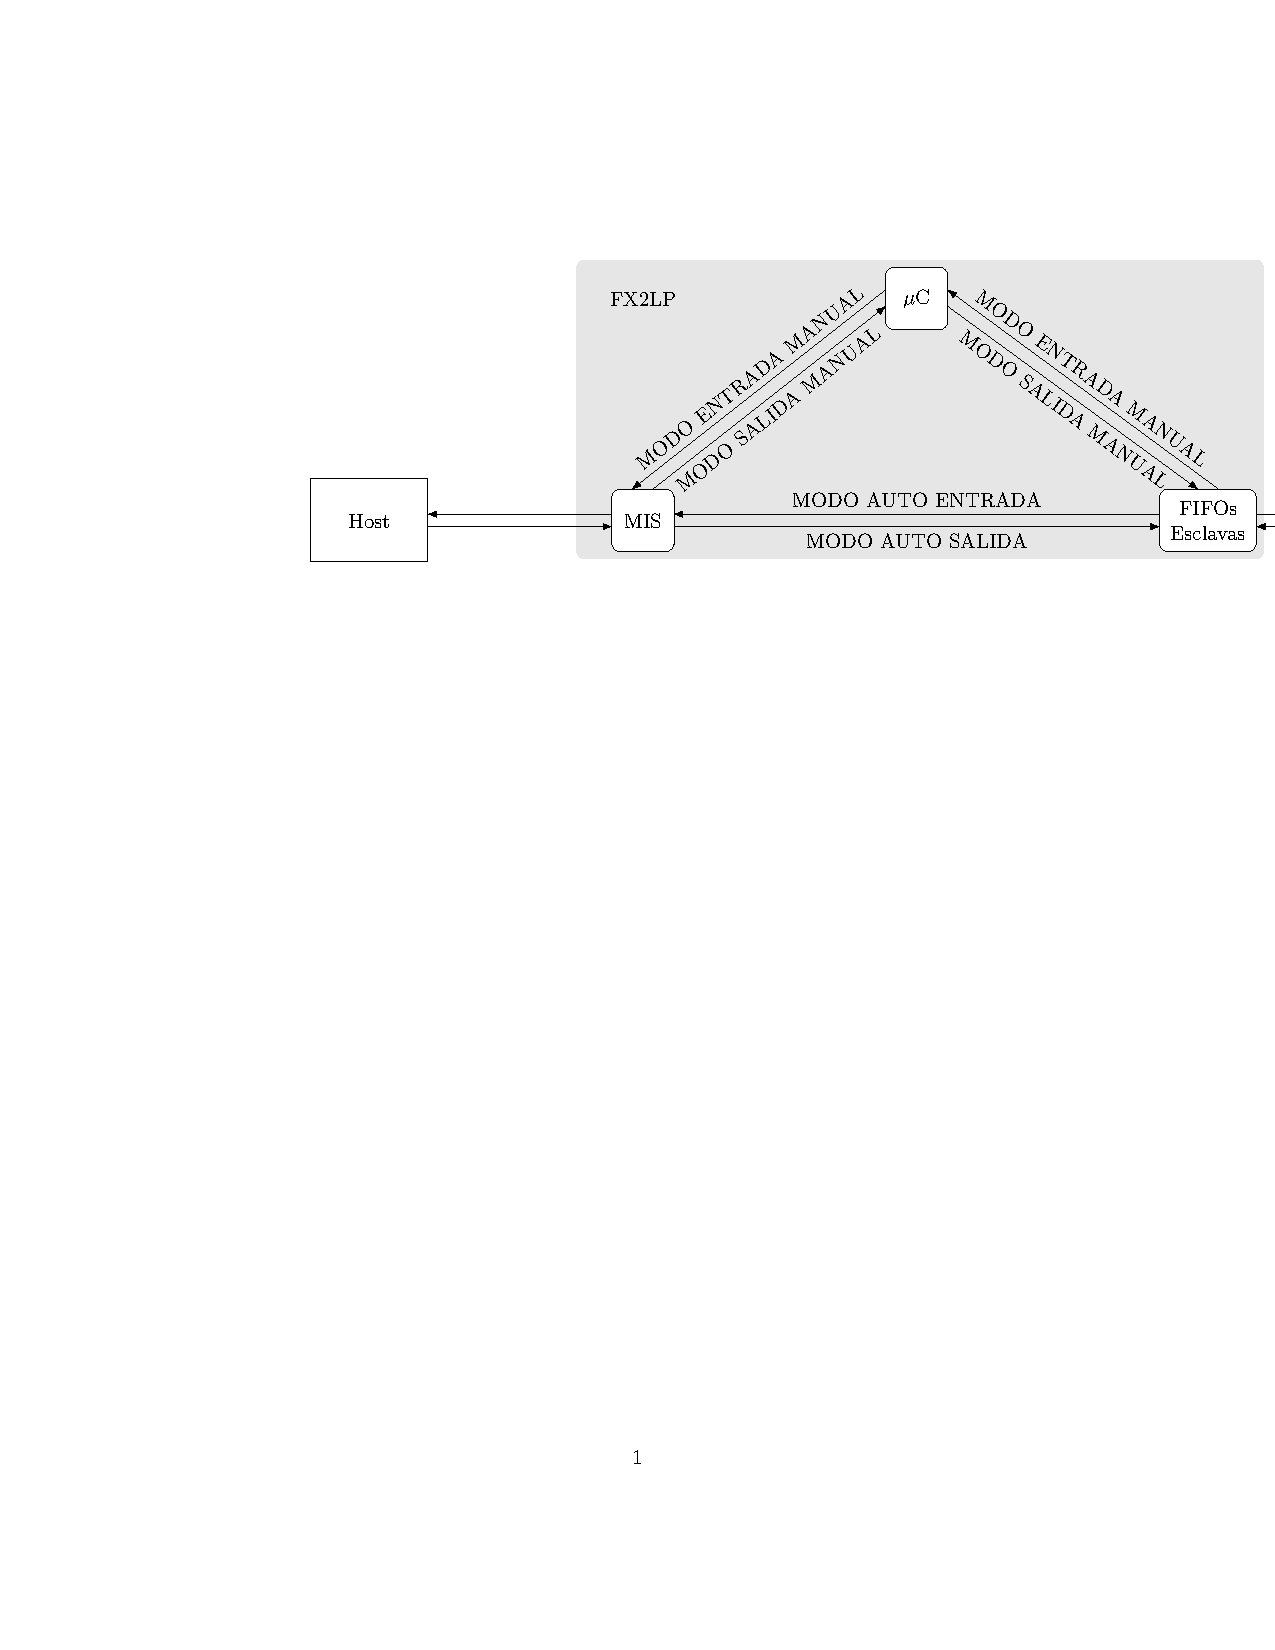
\includegraphics[width = 0.6\textwidth]{tikzImg/esquemafifo}
			\caption{Modos de conexión de la memoria FIFO, el microntrolador y el MIS}
			\label{modesfifo}
		\end{figure}
	
	\subsection*{Memoria FIFO}
		Al poseer el sistema un MIS, que es un serializador de datos, el sistema usa la memoria FIFO como buffer.%la memoria FIFO de 4kB es usada por el sistema como buffer.
		Se conecta de forma directa a los periféricos y es configurable, lo que permite al usuario disponer del espacio conforme requiera las necesidades de ancho de banda para los sistemas diseñados, evitando así las congestiones en casos de mucho flujo de datos. En el otro extremo, puede ser conectada al tubo USB o al microcontrolador, dirigiendo los datos directamente a la PC o realizando alguna acción sobre ellos antes de enviarlos, respectivamente. Cada uno de estos modos son configurables de forma independiente tanto para los paquetes entrantes como salientes.\\
		
		En la Figura \ref{modesfifo} se grafica lo anterior. Cypress denomina MODO AUTO ENTRADA a los datos que se dirigen desde un periférico hacia anfitrión, de forma directa sin pasar por el microcontrolador. De forma análoga, los datos que salen del anfitrión y no pasan por el 8051, lo hacen en MODO AUTO SALIDA. Cuando los datos pasan por el microcontrolador, se utiliza el MODO MANUAL. Cabe notar que los modos de ENTRADA o SALIDA poseen como referencia el anfitrión debido al carácter central que posee éste en la arquitectura USB.\\
		
		
		El sistema FX2LP permite configurar los buffers conforme la se ve en la Figura \ref{epconfigs}. Cada buffer tiene una dirección de memoria asignada y corresponde a cada uno de los extremos posibles. Es de destacar que en cualquiera de las configuraciones posibles, se tiene al menos dos buffers. Los diseñadores del integrado pensaron esto como una solución a la congestión. Para ello, los buffers se pueden configurar duplicados, triplicados o cuadruplicados, dependiendo de las necesidades. Luego, el sistema de forma automática se encarga de permutar los buffers, reasignando los espacios de memoria al lugar físico del circuito donde se puedan almacenar nuevos datos, de forma tal que no queden datos retenidos en el dispositivo maestro. Cómo se detallará más adelante, para este trabajo se configuraron dos extremos como el modo 11 de la Figura \ref{epconfigs}, es decir, un extremo con 3 buffers de 1024 bytes y otro con 2 buffers de 512 bytes.\\
		
		Los buffers pueden ser conectados directa hacia el MIS para realizar una comunicación automática entre la PC y los periféricos, estableciendo una cantidad umbral de datos que, cuando se rebasa, envía los datos hacia la PC; o bien se puede acceder a ellos desde el microcontrolador, leer, chequear y/o editar los datos antes de enviar hacia la PC o los periféricos.\\
			
		\begin{figure}[h]
			\centering
			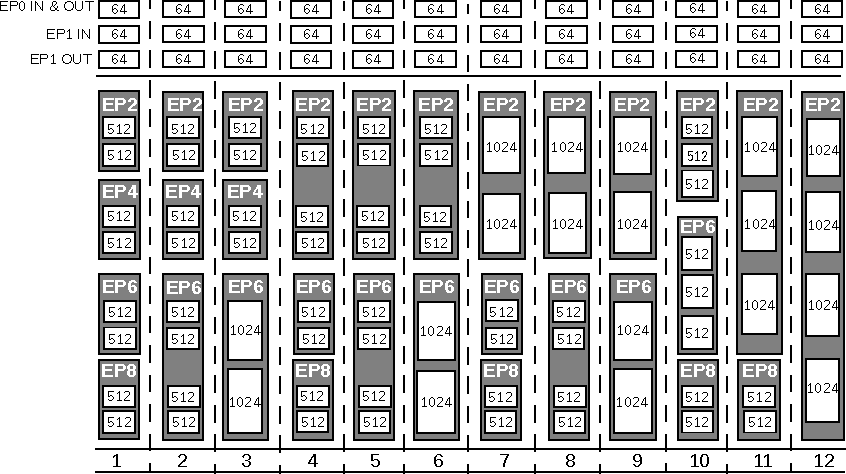
\includegraphics[width=0.6\textwidth]{bufconf}
			\caption{Configuraciones admitidas para los buffers de periféricos}
			\label{epconfigs}
		\end{figure}